\subsection{Results when introducing second shepherd}
The implementation of a second shepherd introduces an additional dog whose task is the guide the sheep towards the target. Figures \ref{fig:single-shepherd} and \ref{fig:second-shepherds} illustrate the results for trajectories with one and two shepherds. A distance penalty of 0.05 was applied. As planned, the introduction of a second shepherd is evident, and it appears to follow a trajectory similar to that of the initial shepherd but at a higher speed. Further evaluation is needed to determine whether this is always the case.

\begin{figure}[!h]
    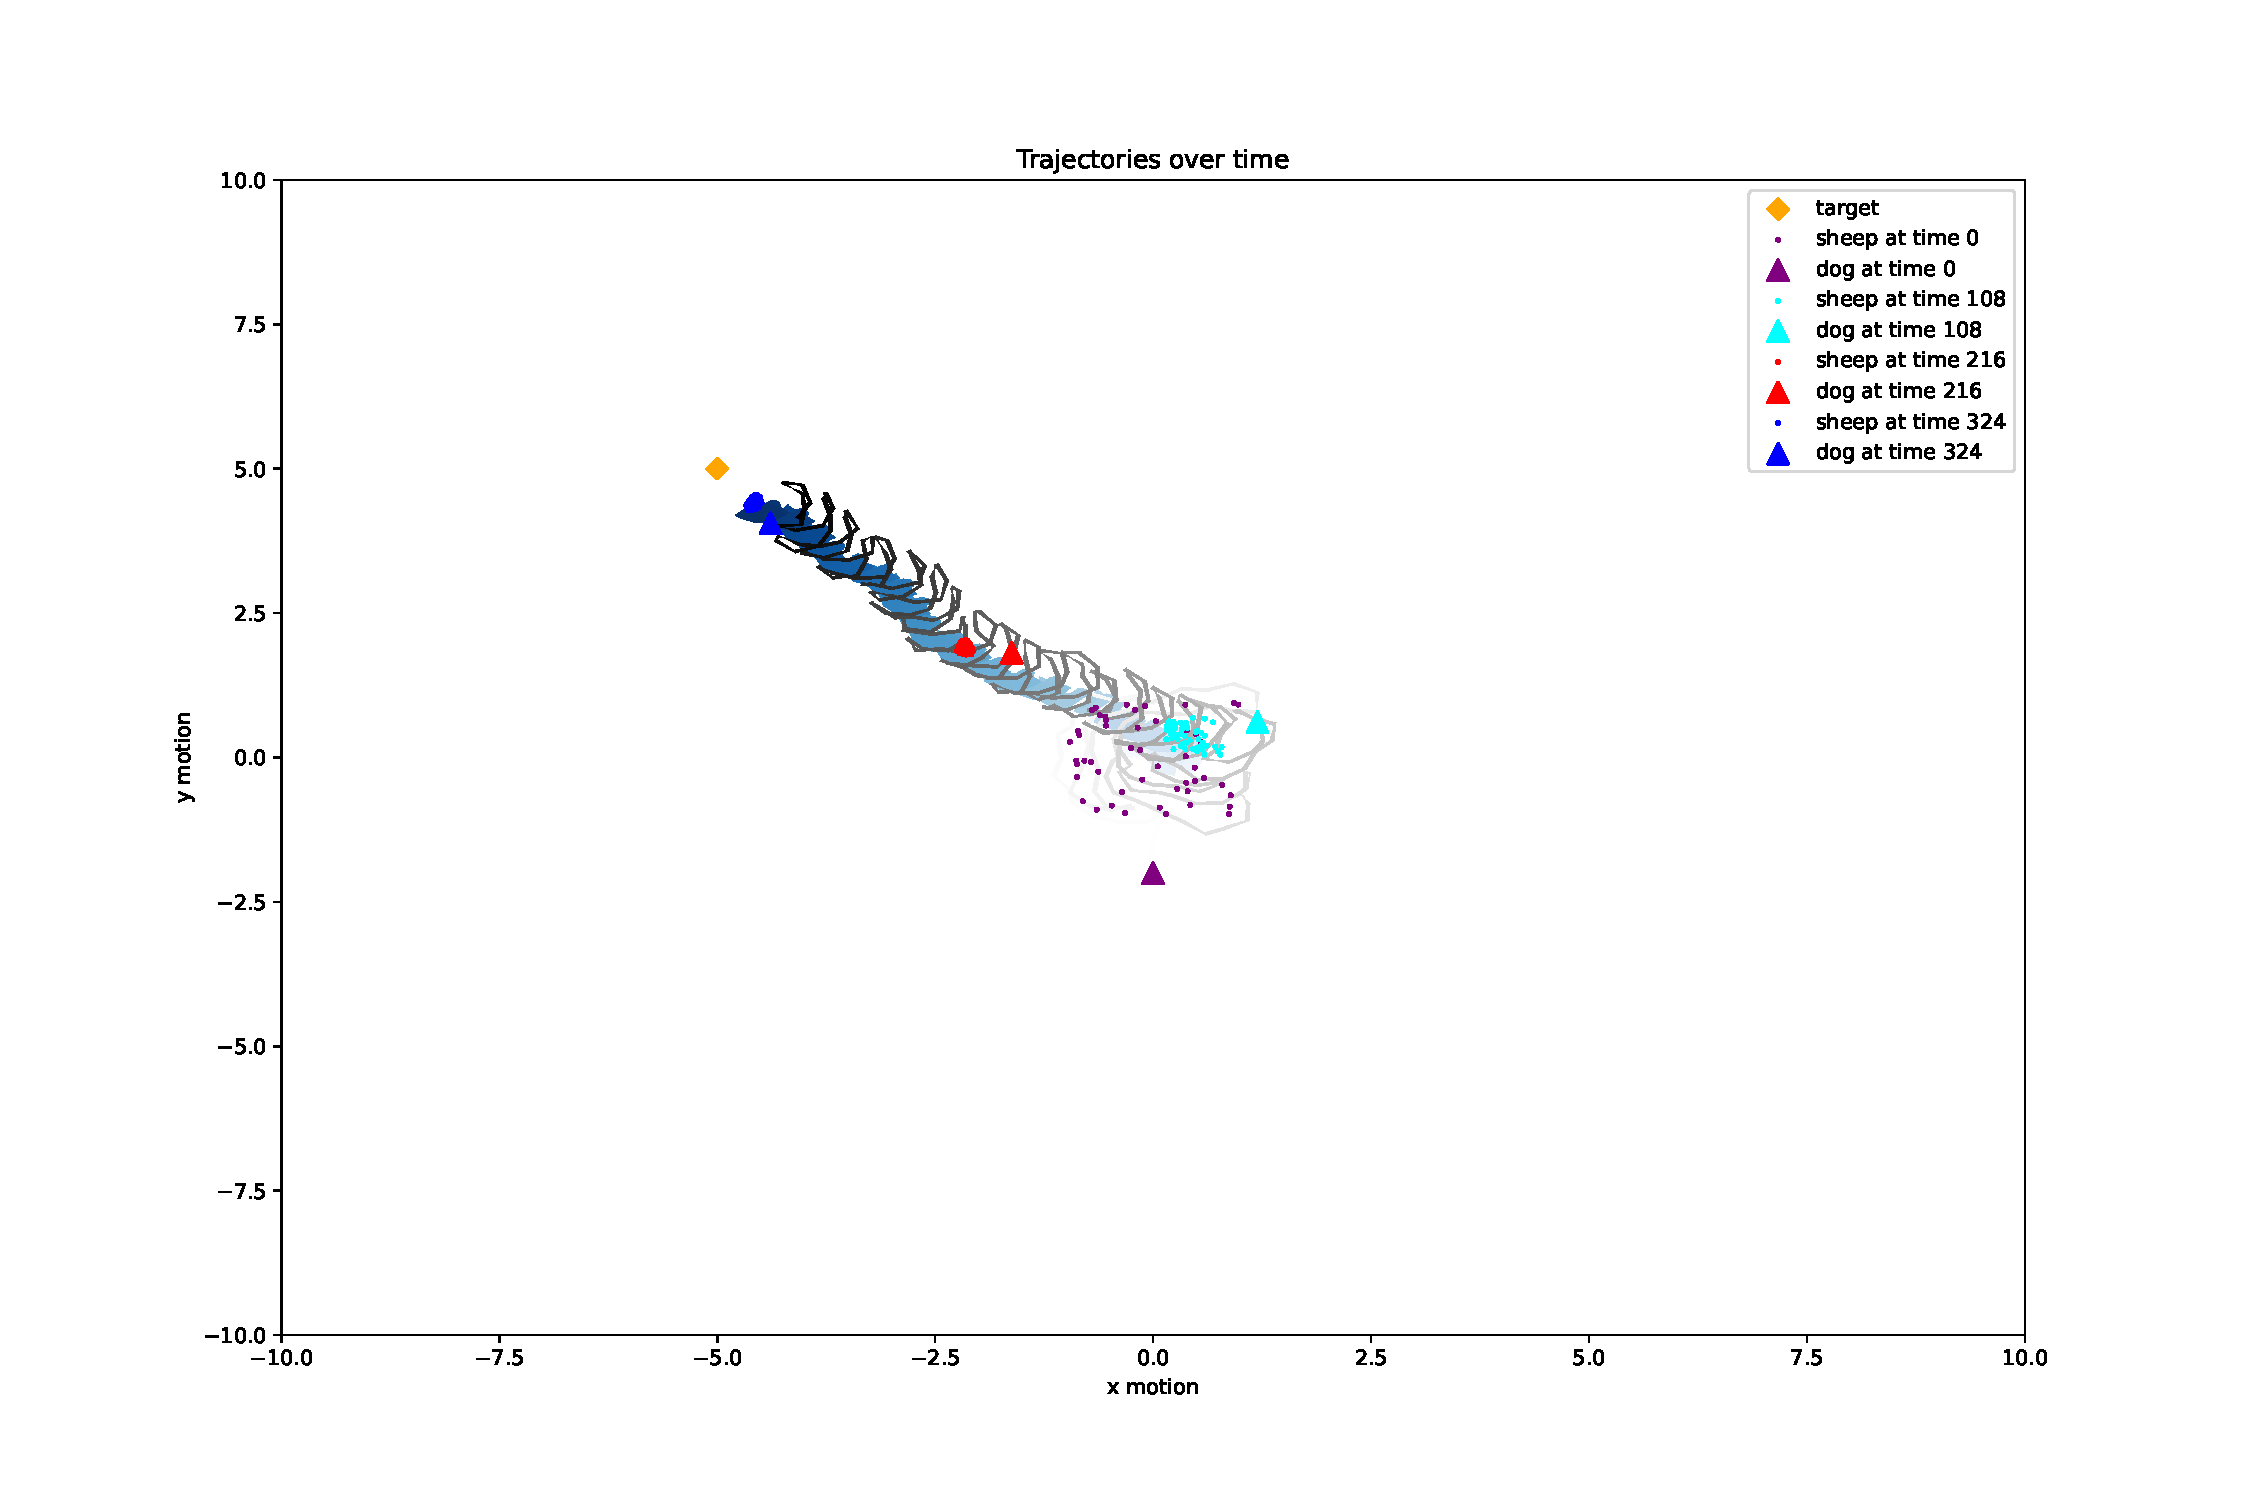
\includegraphics[width=0.9\textwidth]{figures/single-shepherd.pdf}
    \caption{Trajectory plot using a single shepherd}
    \label{fig:single-shepherd}
\end{figure}

\begin{figure}[!h]
    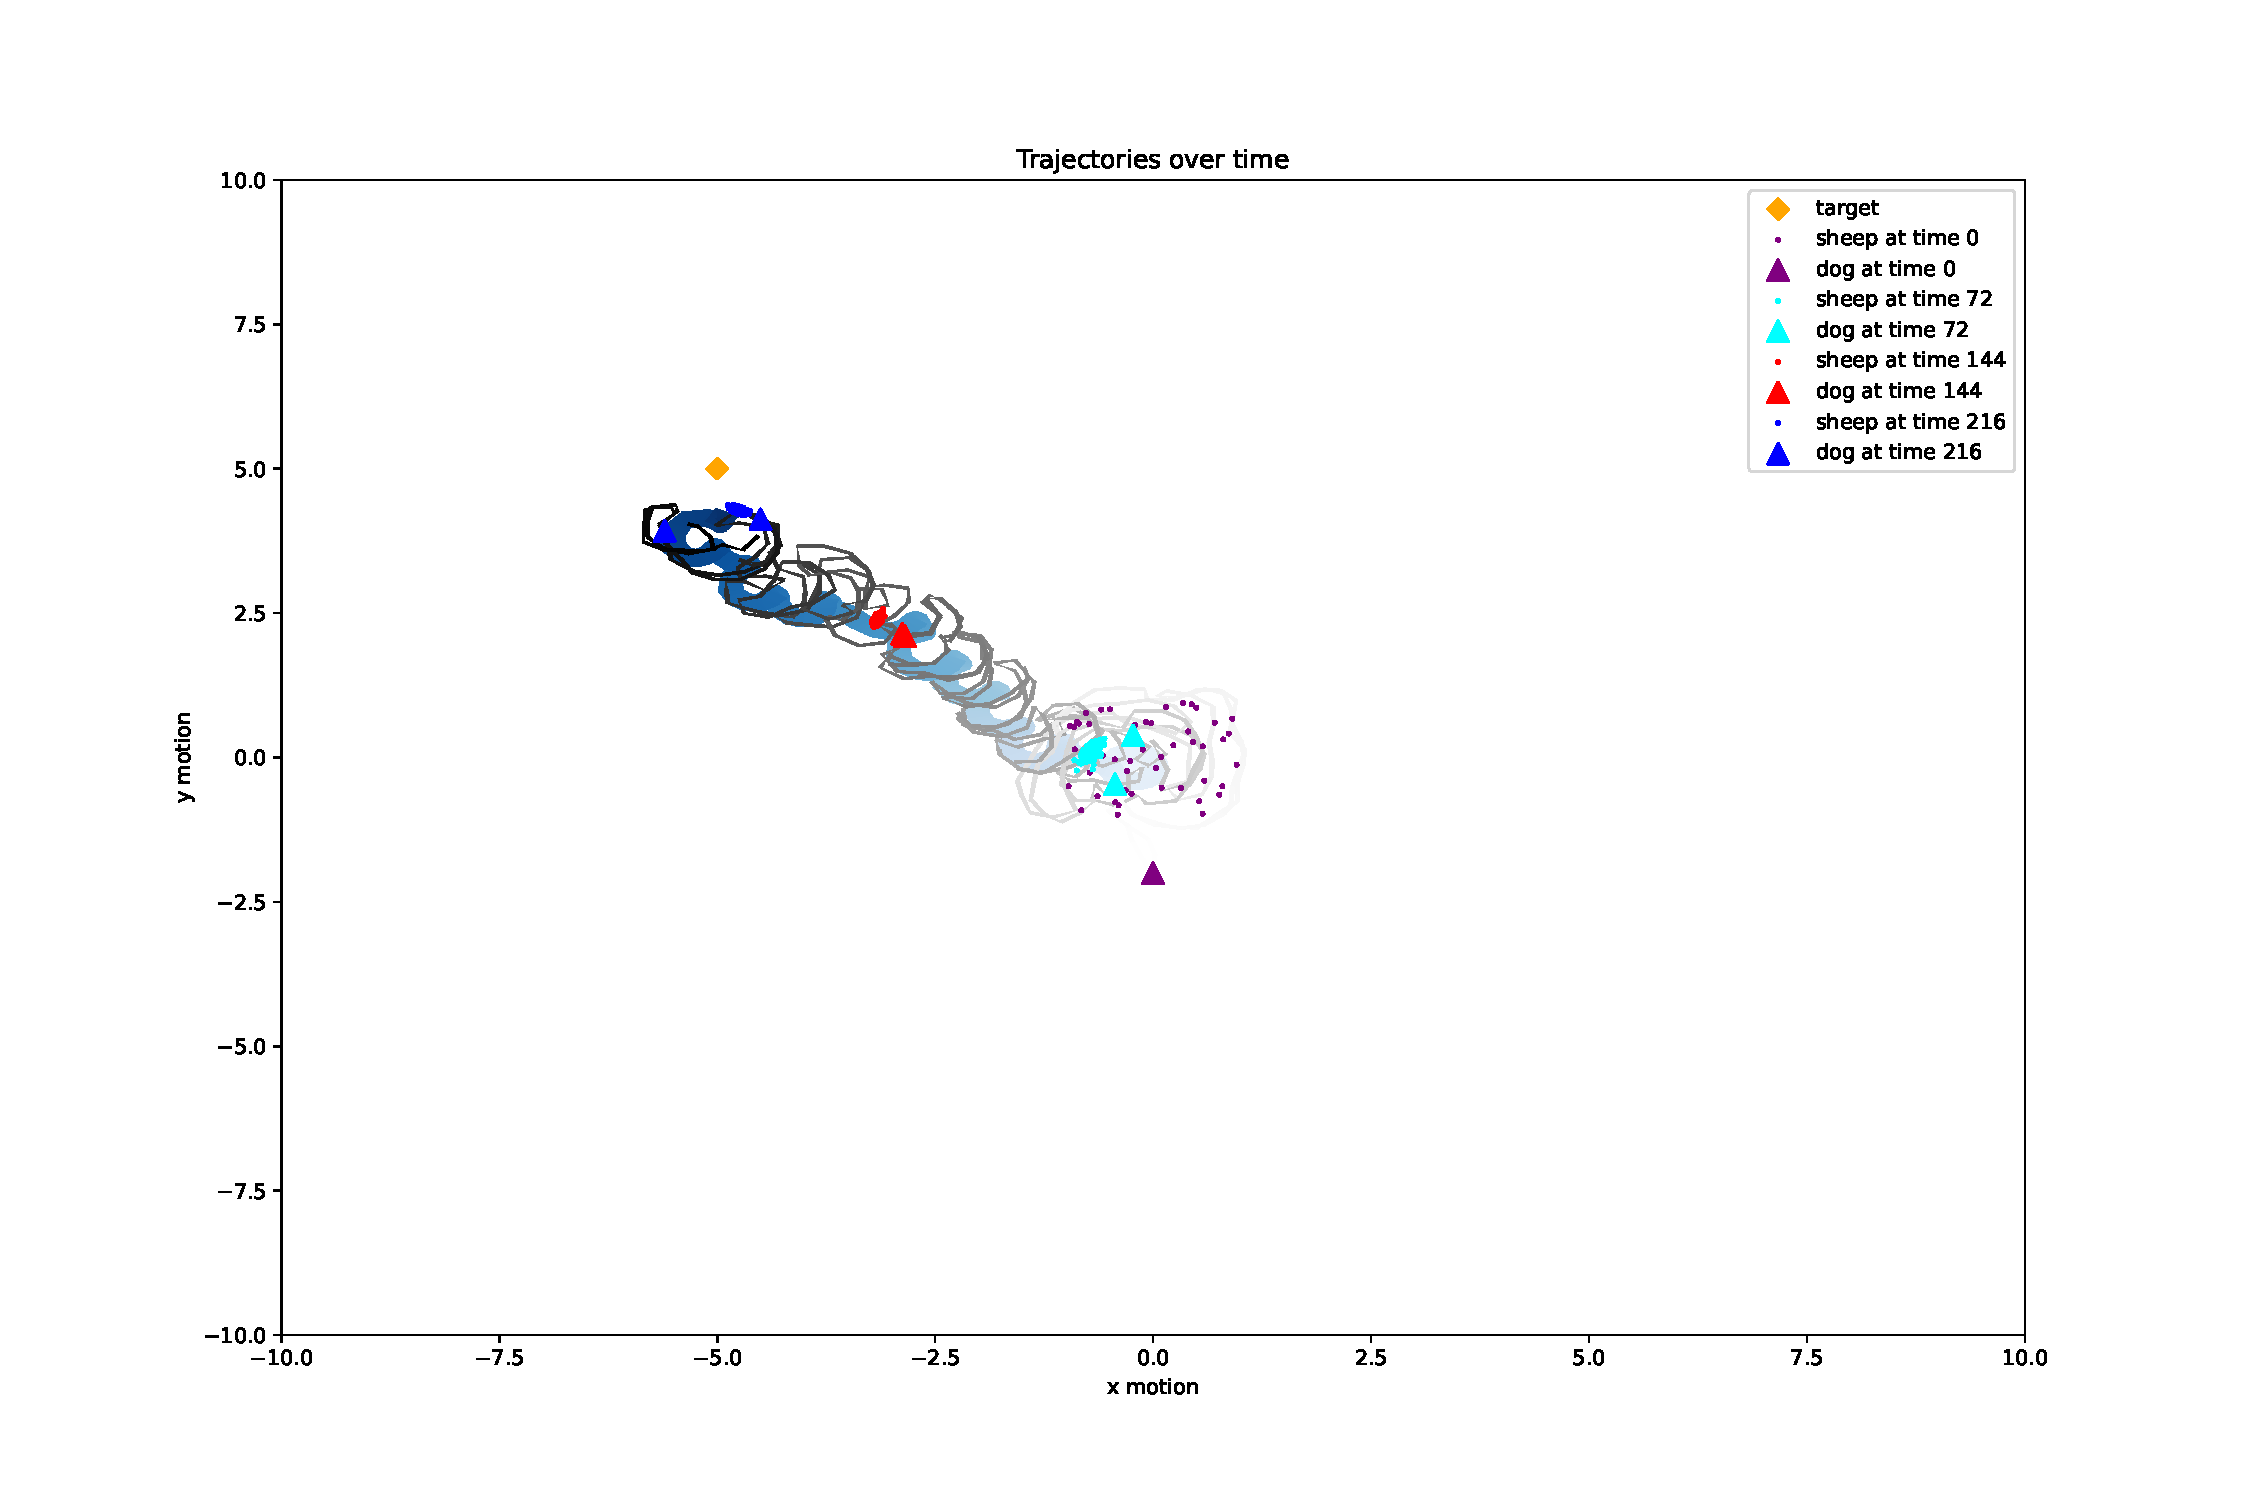
\includegraphics[width=0.9\textwidth]{figures/second-shepherd.pdf}
    \caption{Trajectory plot using two shepherds}
    \label{fig:second-shepherds}
\end{figure}

\newpage


\subsection{Results when introducing a fence}
%%%% TODO: position correctly when all other text has also been added
The implementation of a fence ensures that both the dogs and sheep are surrounded by a boundary and prevents them from crossing it. In the figures below, the outcomes are depicted for the herding style 'driving' with and without a fence. As intended, the presence of the fence effectively confines the sheep and dogs within its boundaries, while the dog still leads the sheep to the target.

\begin{figure}[!h]
    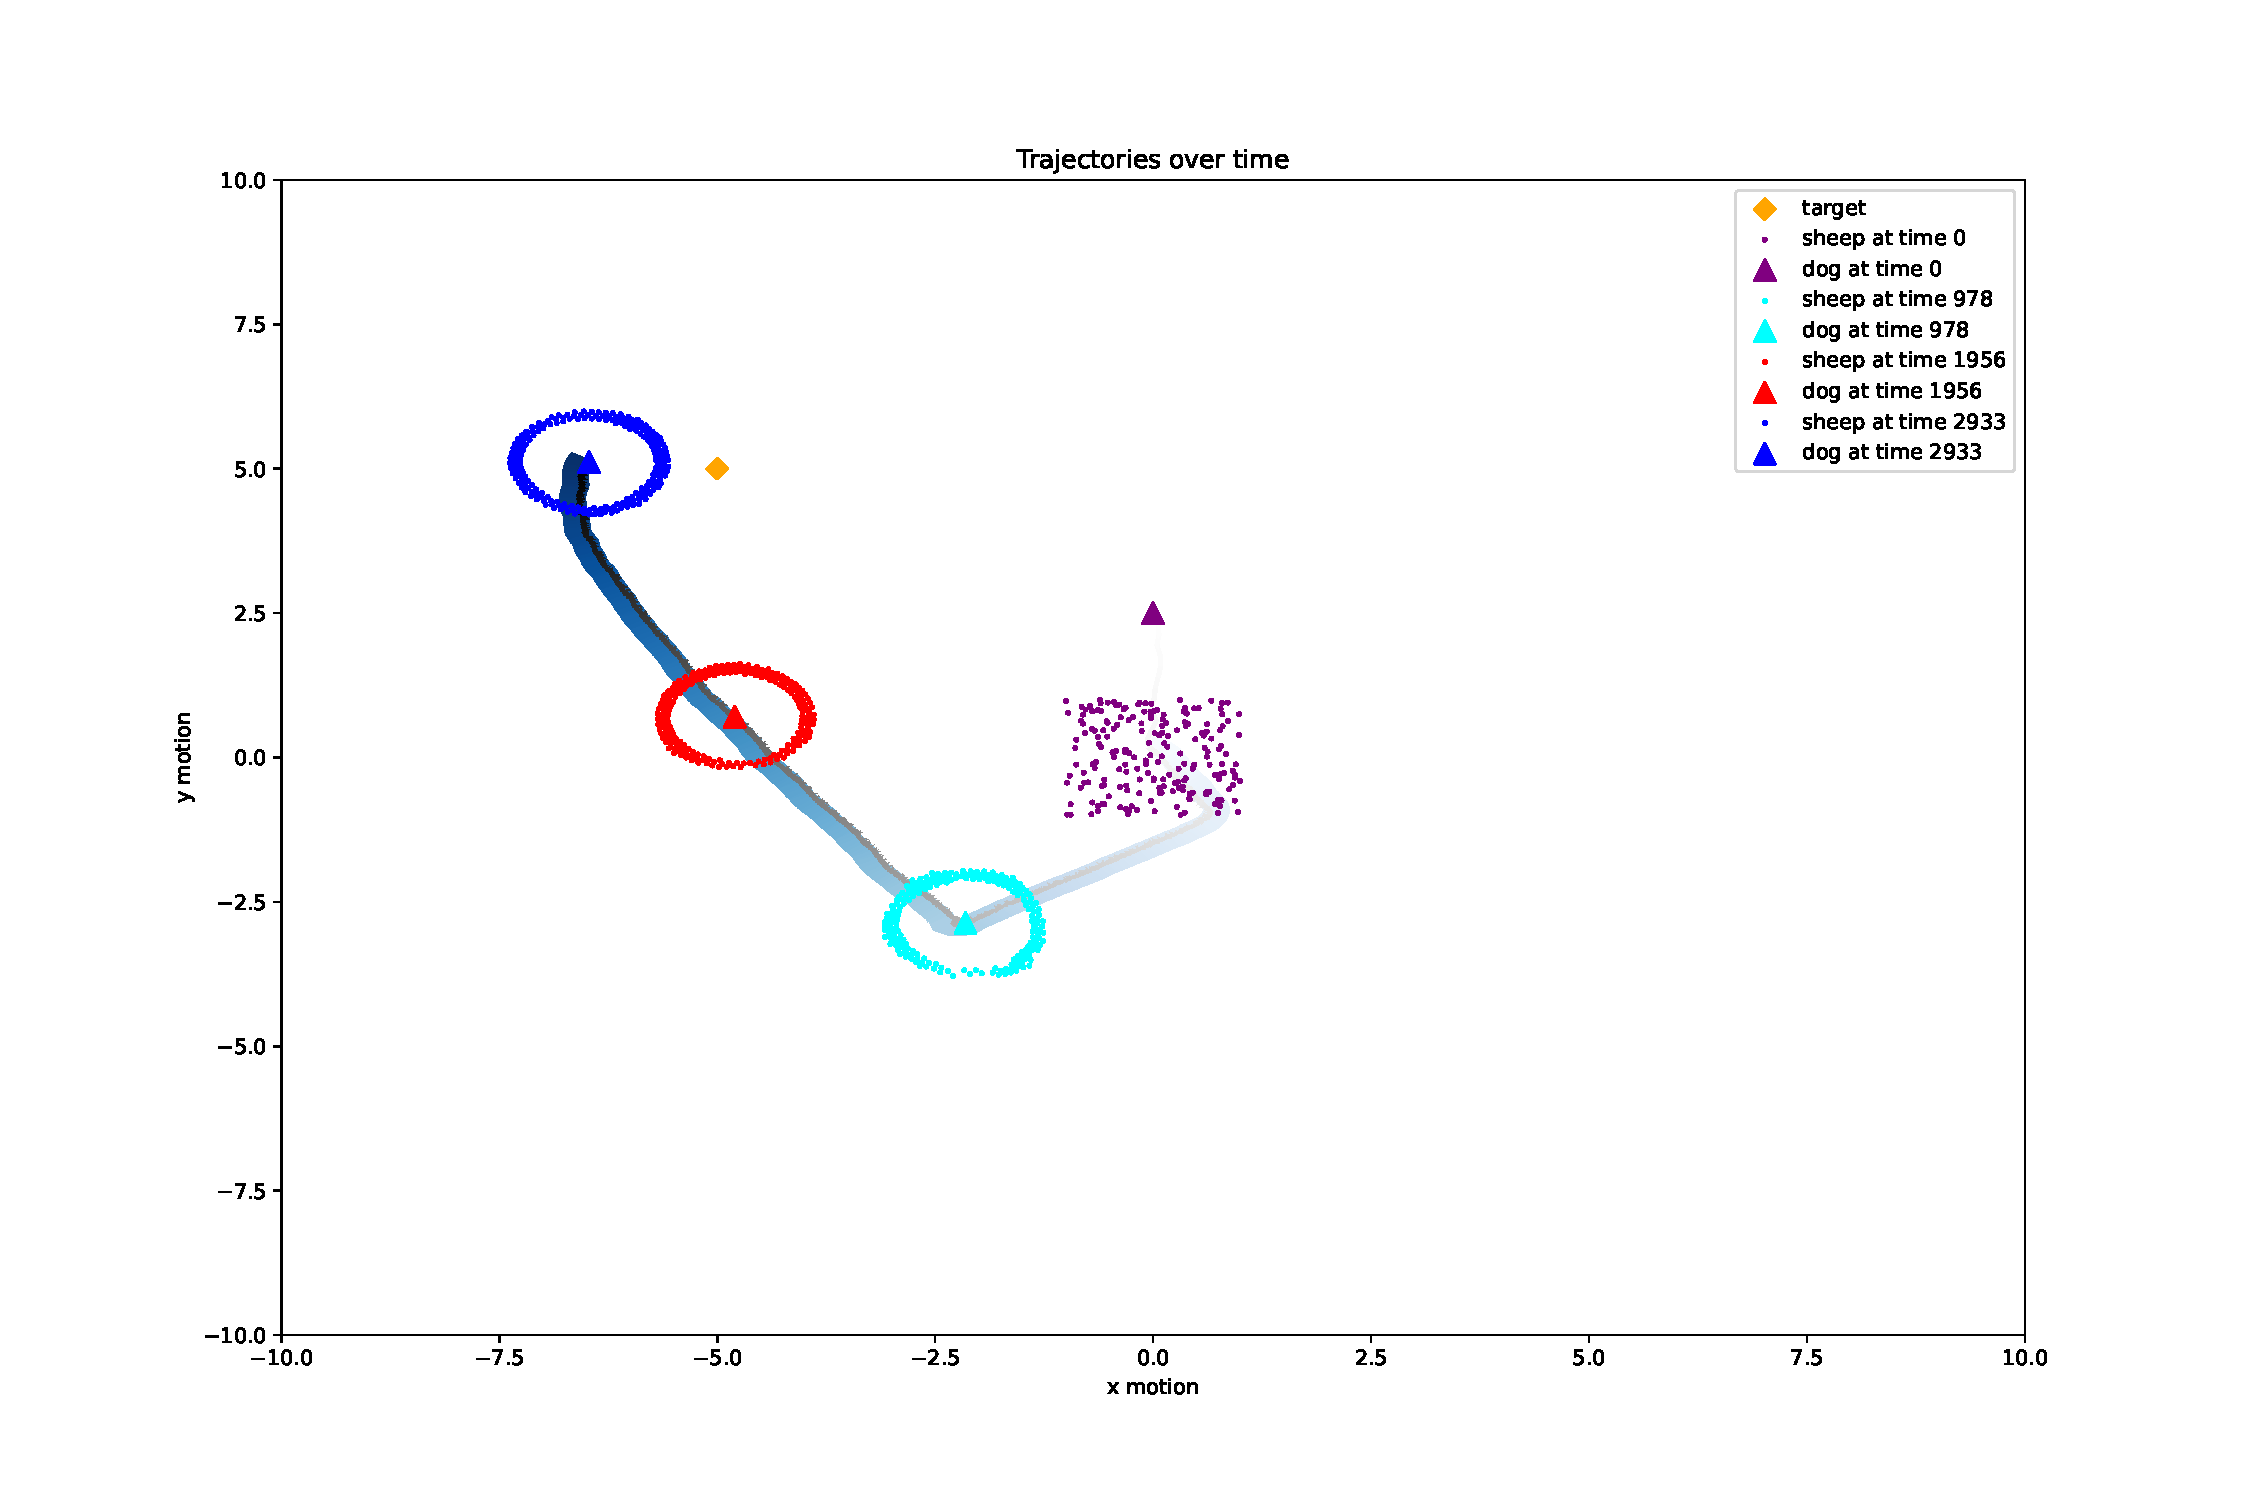
\includegraphics[width=0.9\textwidth]{figures/driving.pdf}
    \caption{Trajectory plot for driving without a fence}
\end{figure}

\begin{figure}[!h]
    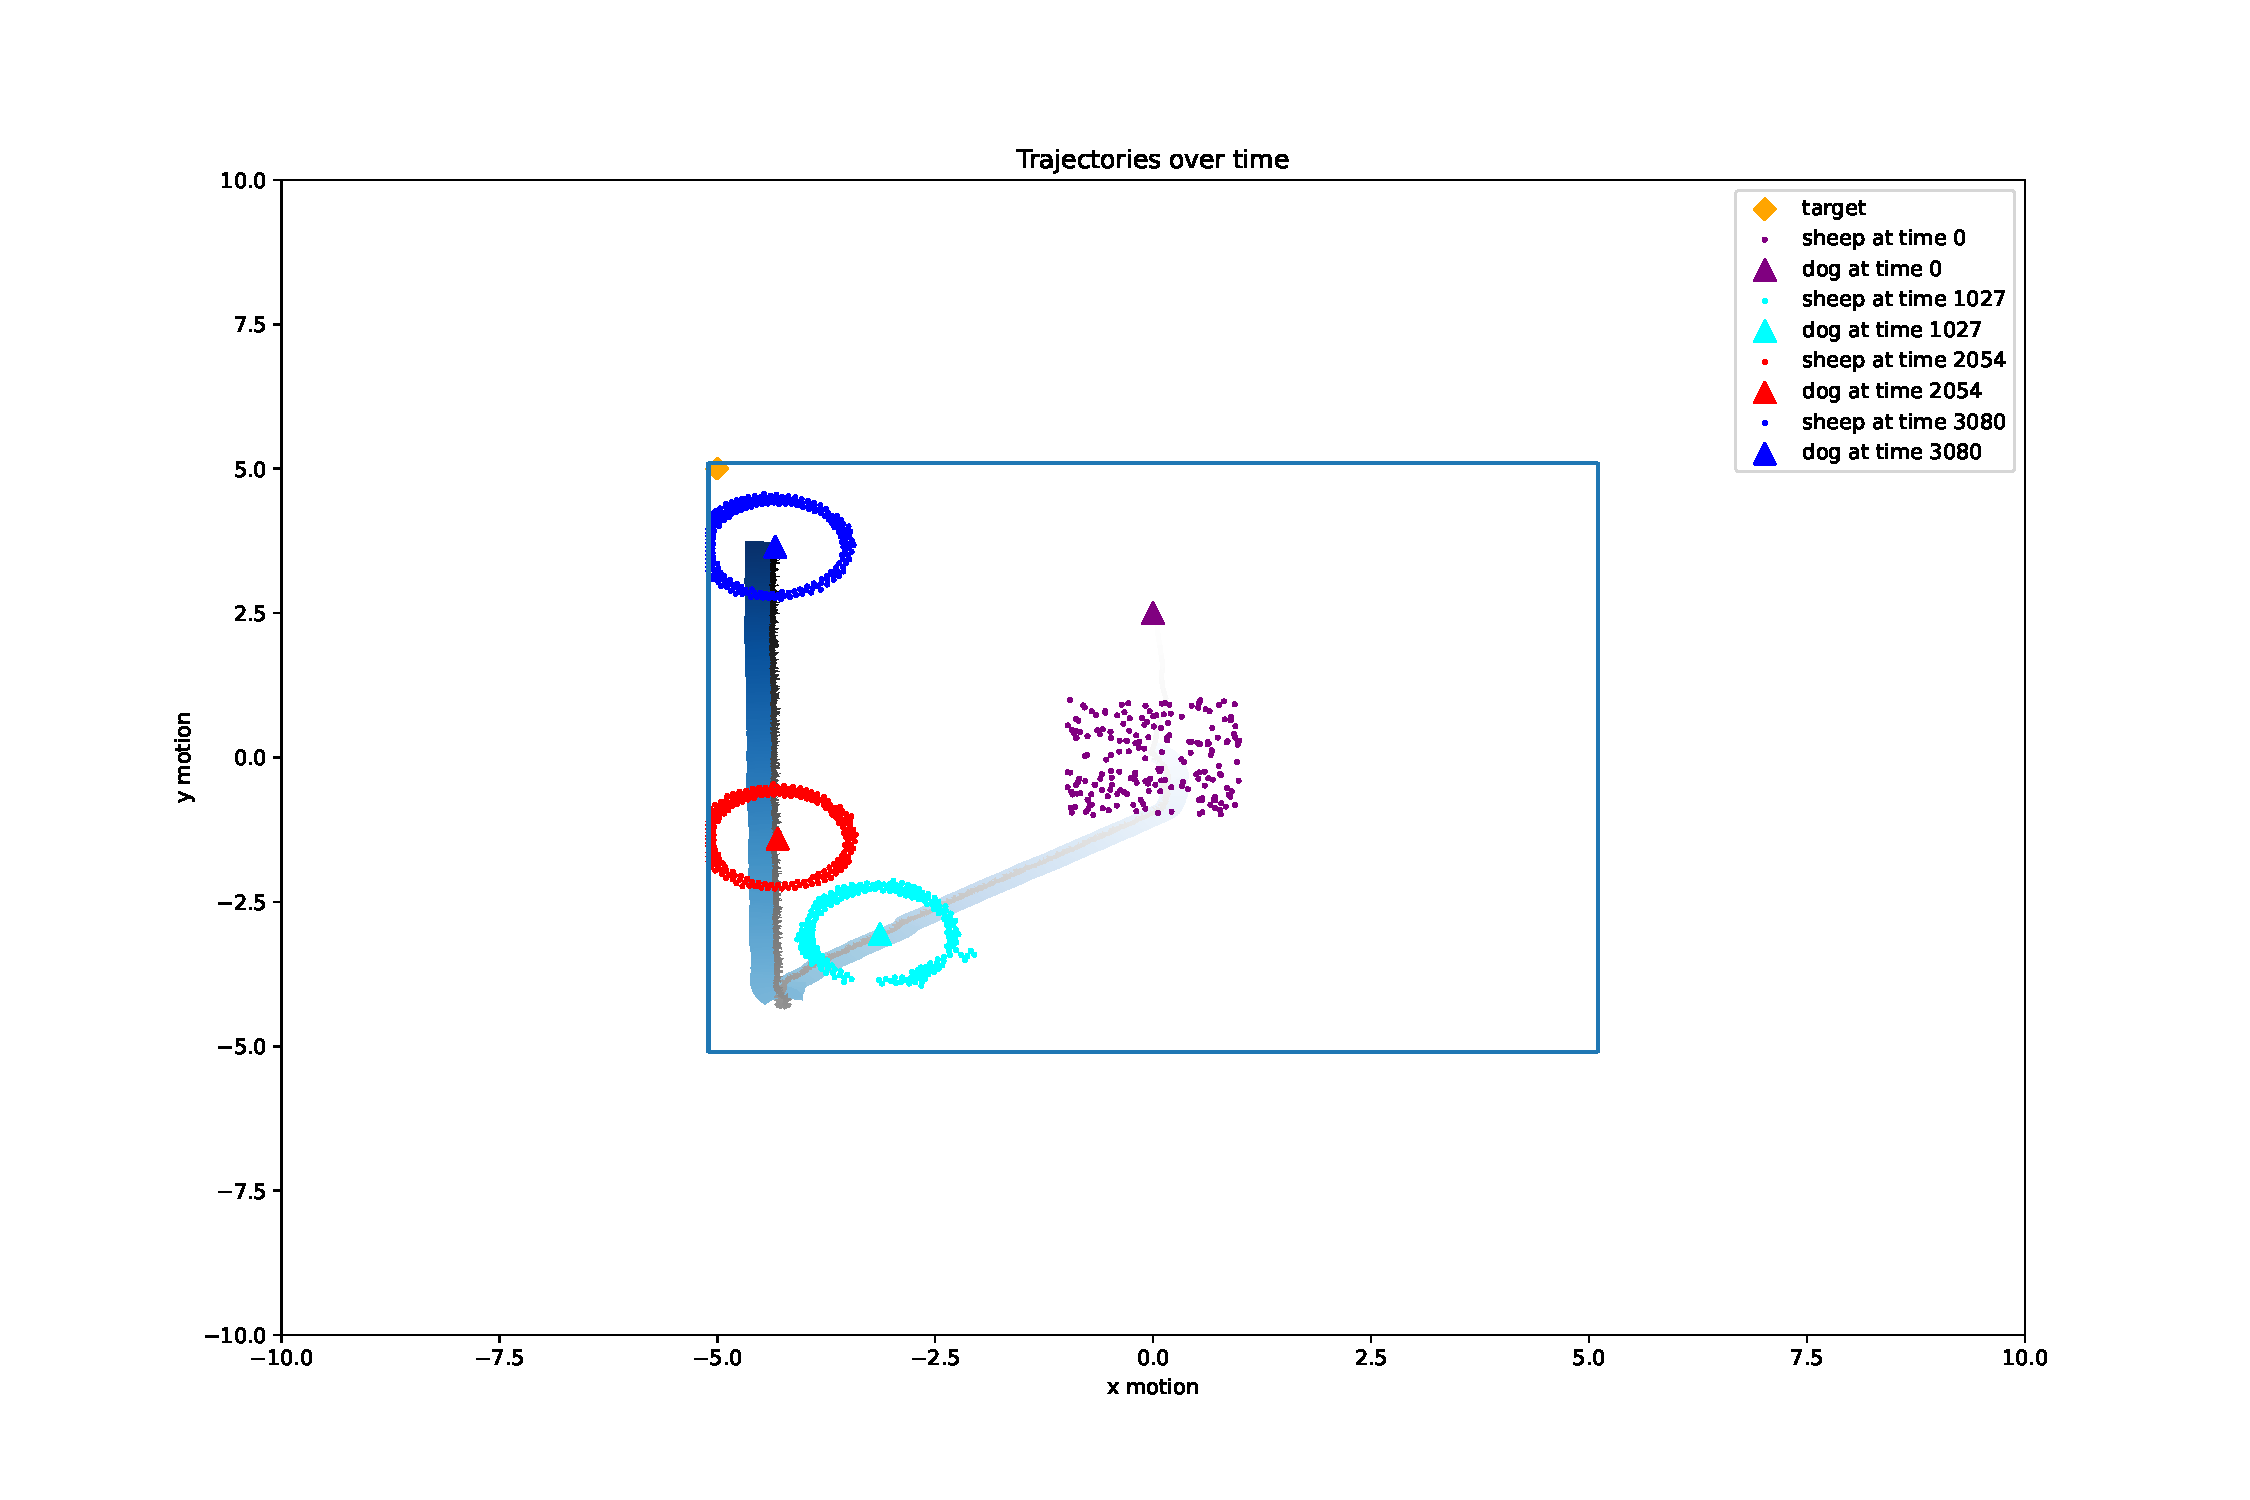
\includegraphics[width=0.9\textwidth]{figures/driving-fence.pdf}
    \caption{Trajectory plot for driving with a fence}
\end{figure}

\newpage


%%% TODO: either include in appendix or leave out
% \begin{figure}[!h]
%   \centering
%   \begin{minipage}[b]{0.49\textwidth}
%     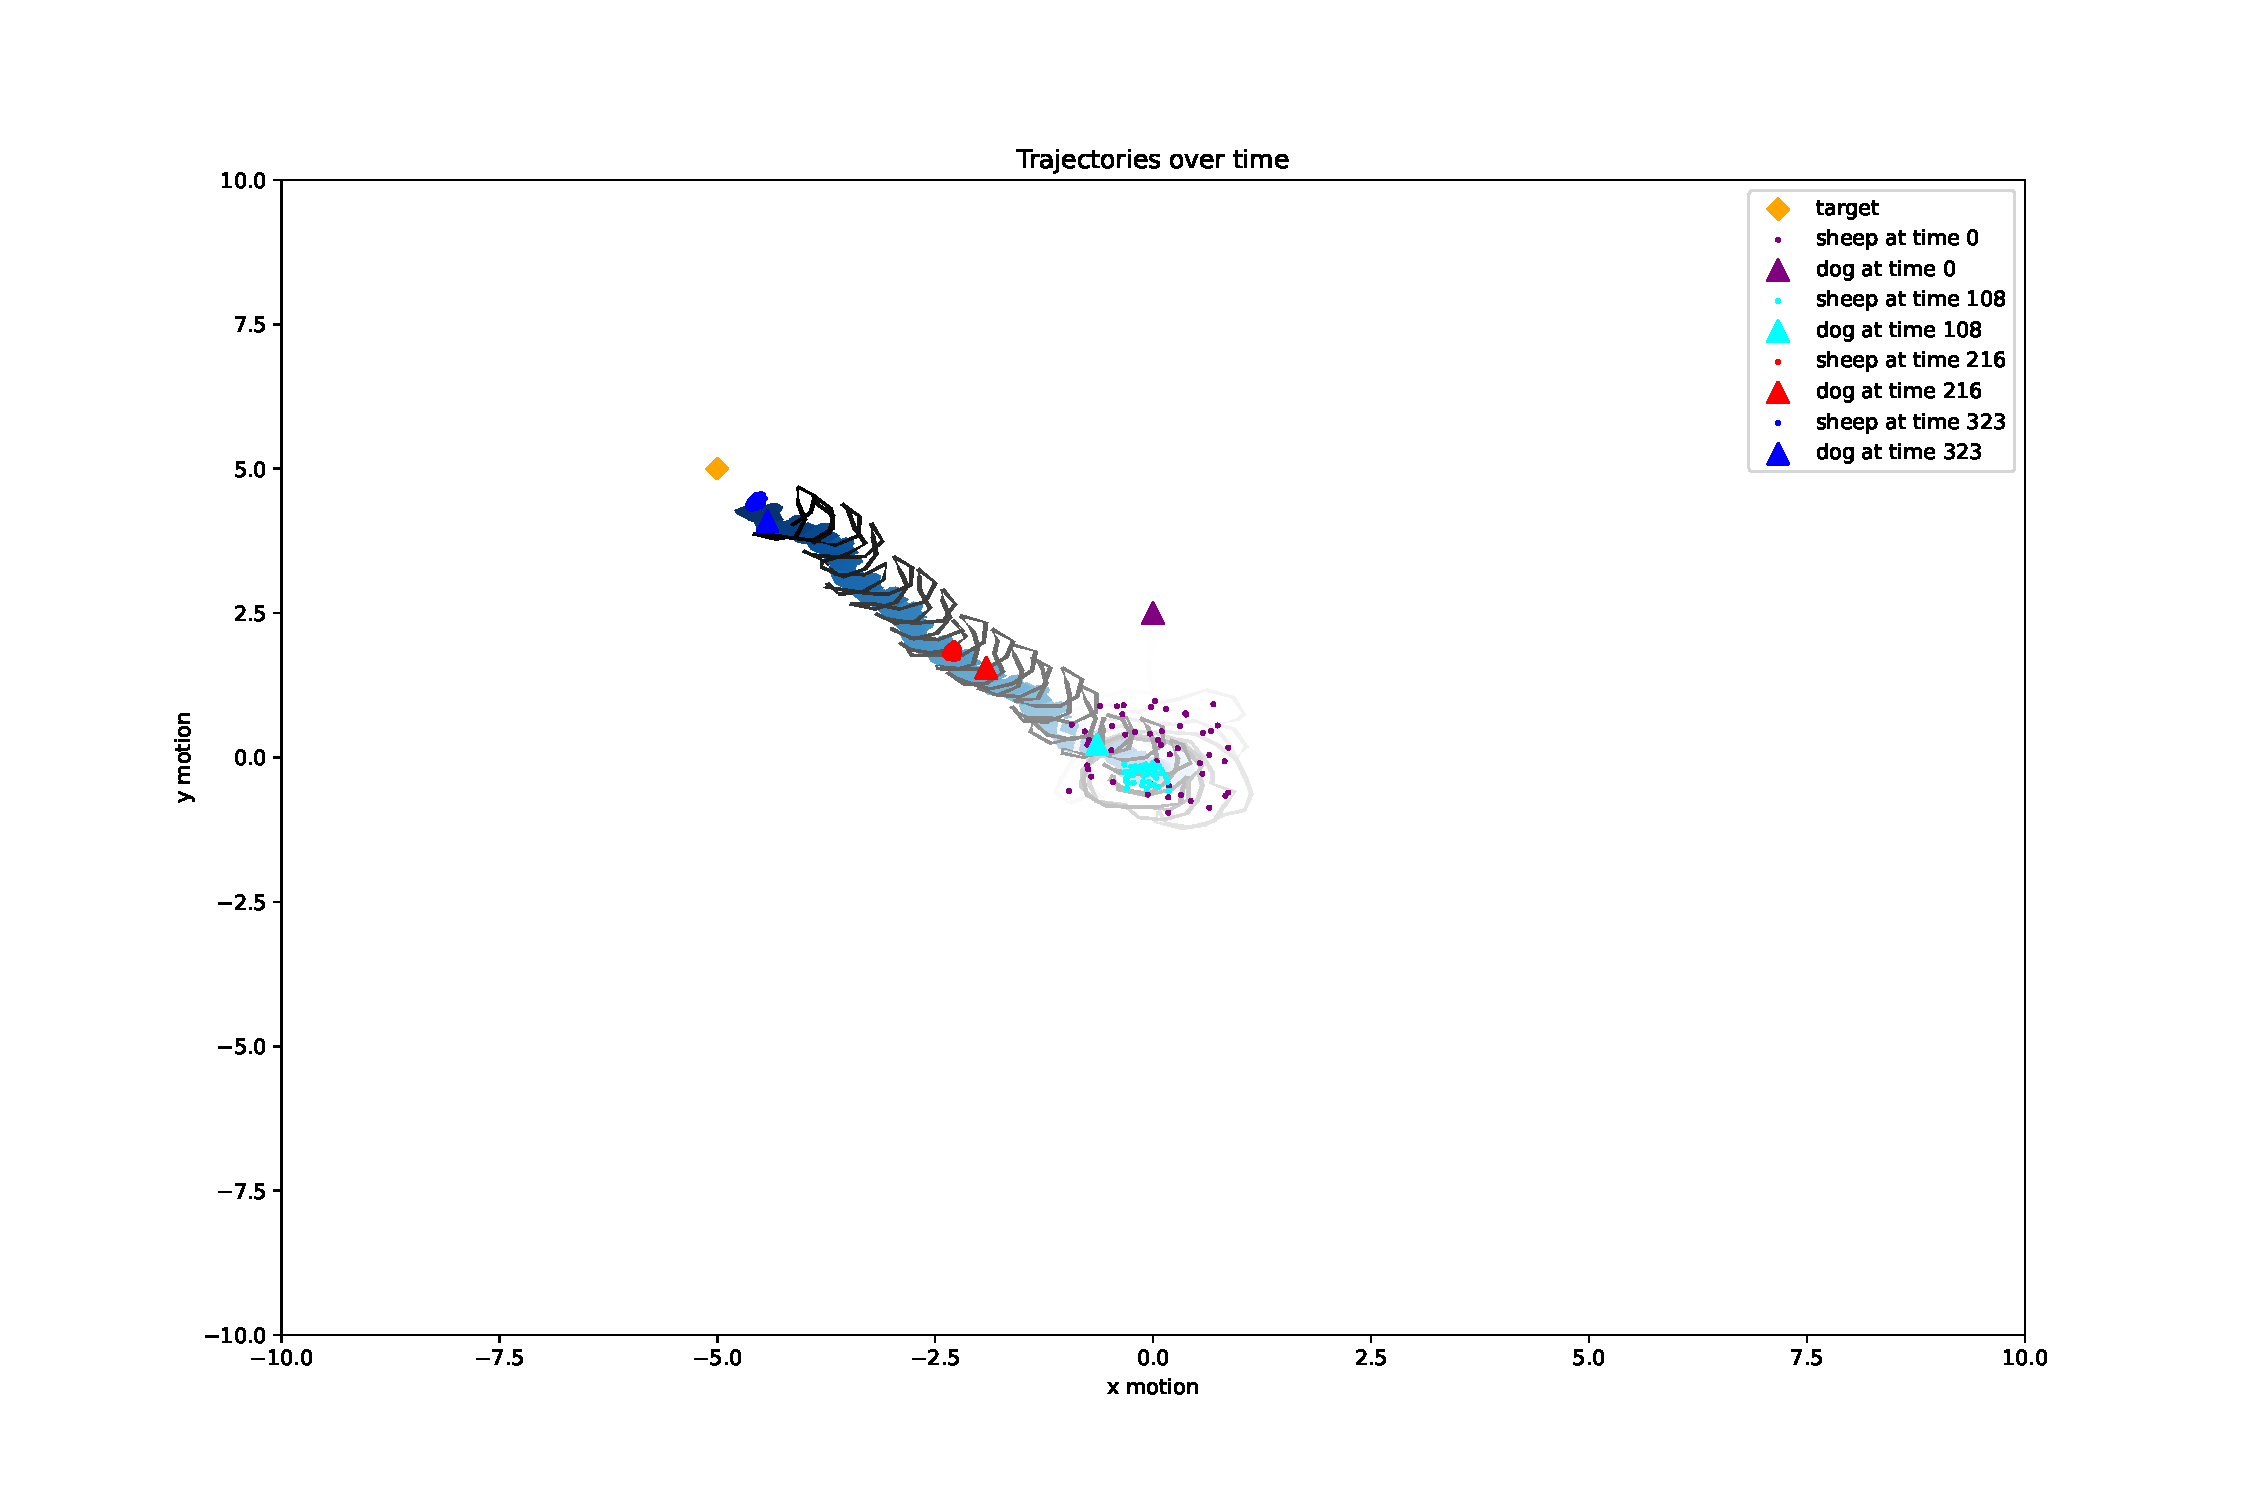
\includegraphics[width=\textwidth]{figures/droving.pdf}
%     \caption{}
%   \end{minipage}
%   \hfill
%   \begin{minipage}[b]{0.49\textwidth}
%     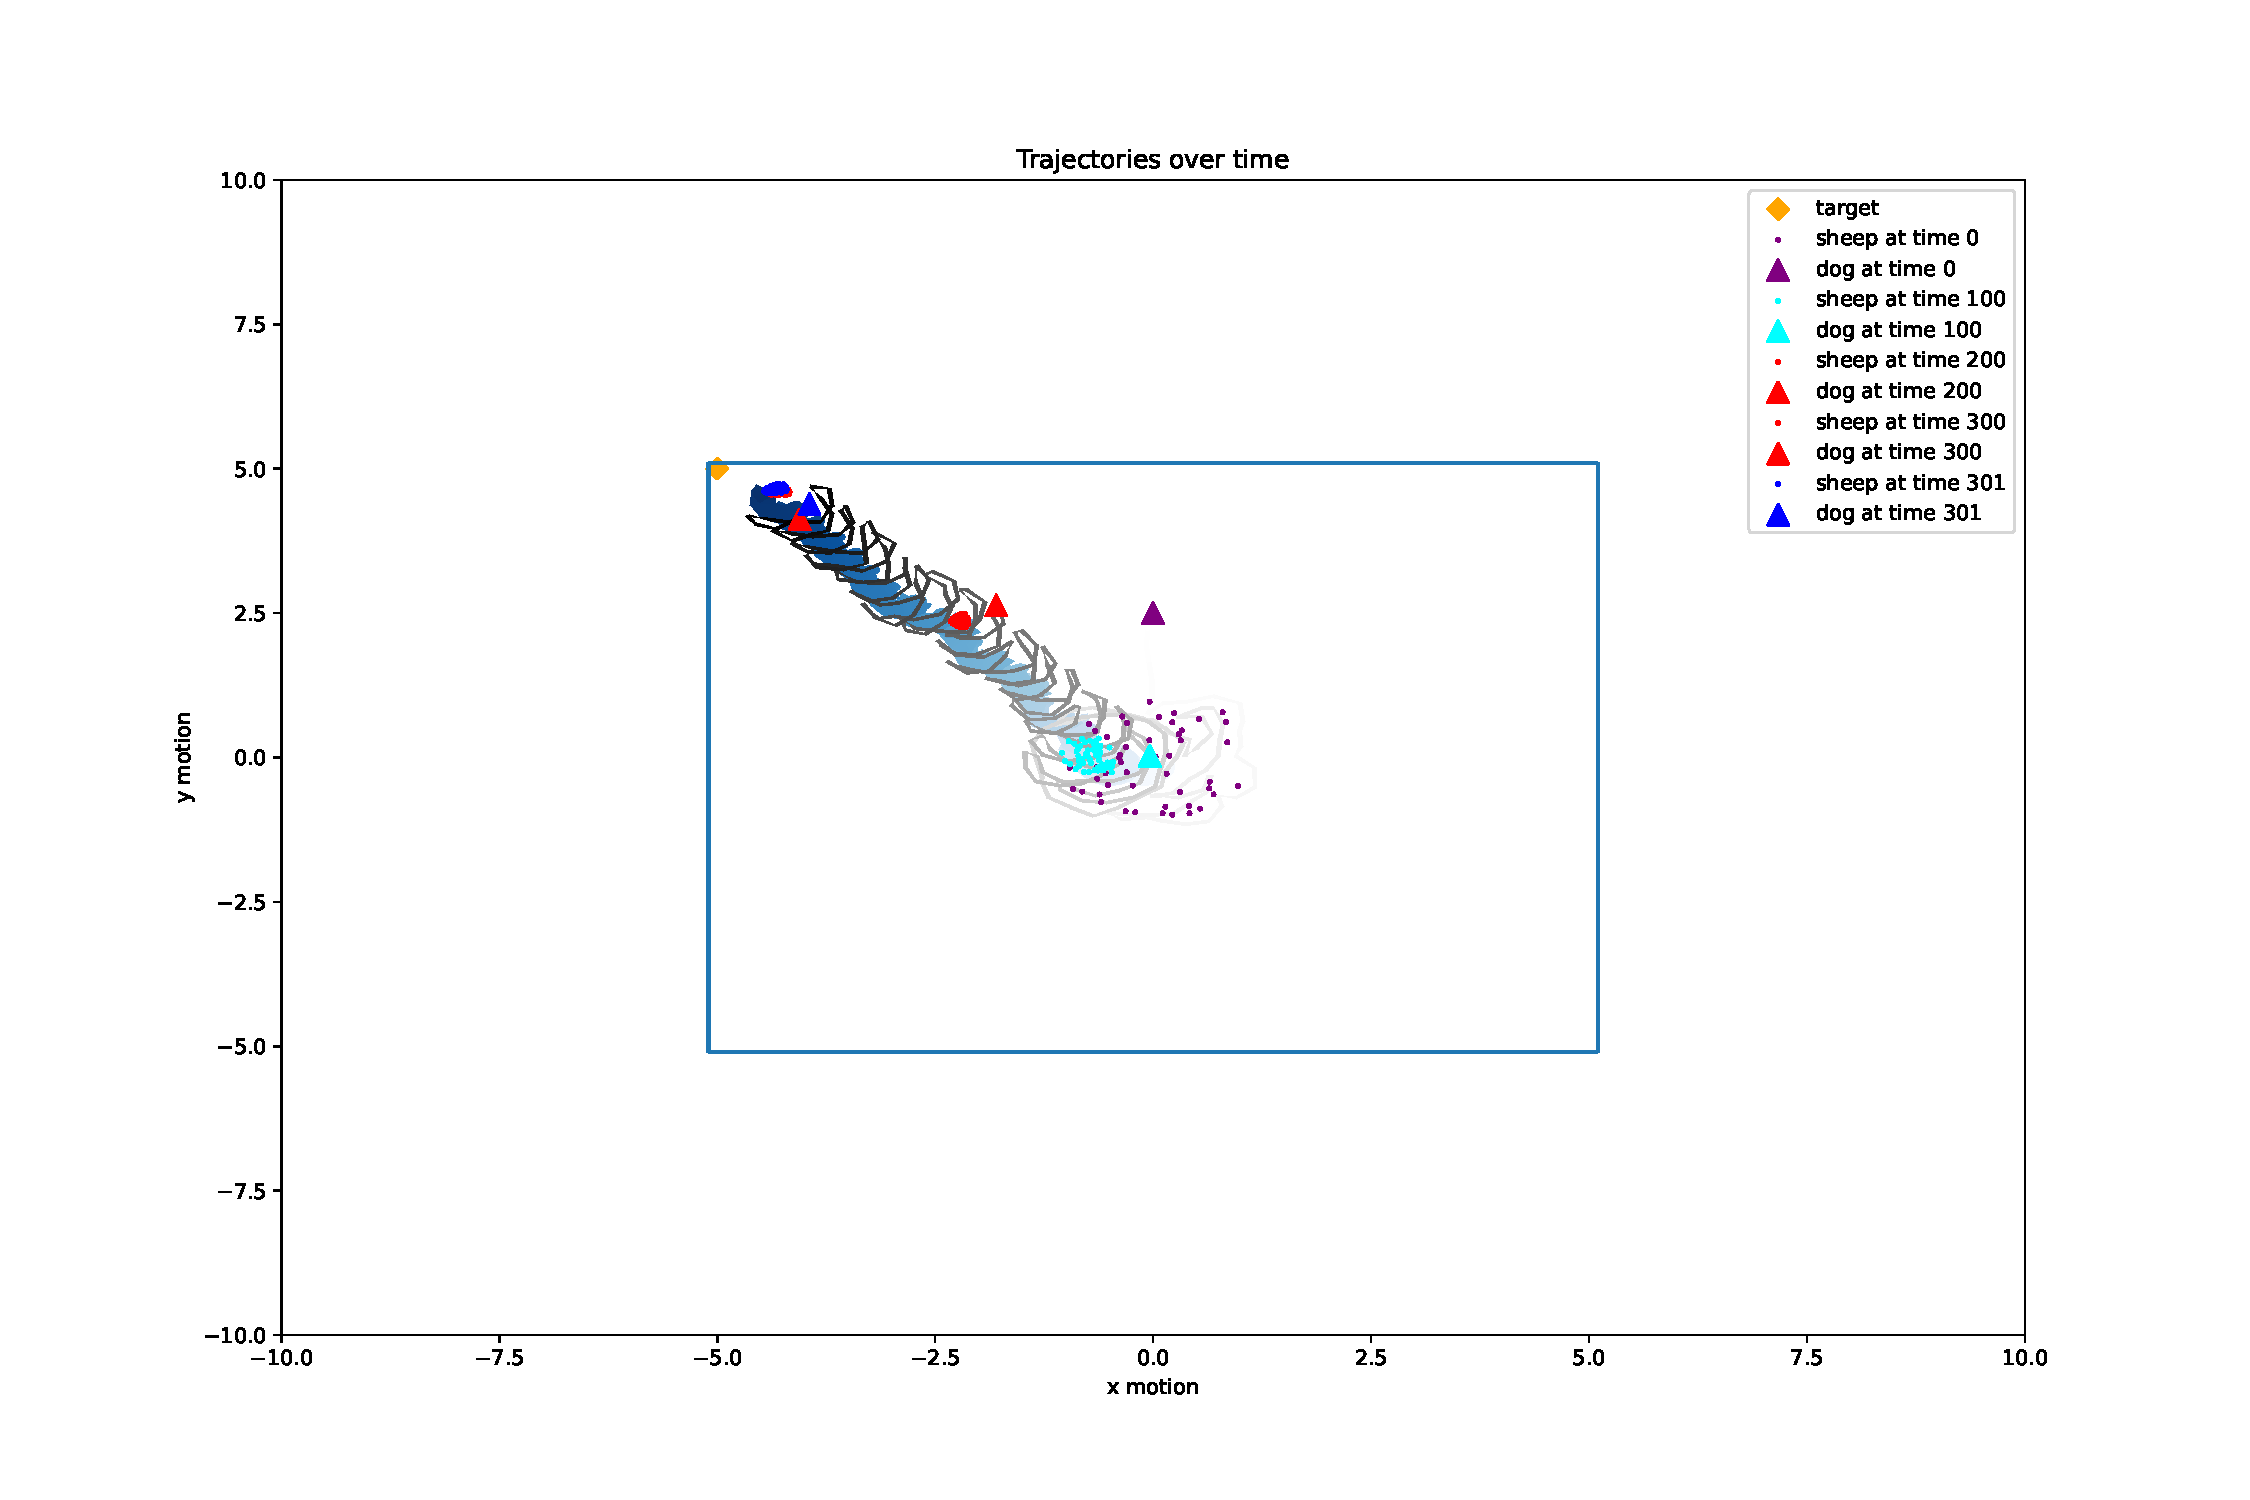
\includegraphics[width=\textwidth]{figures/droving-fence.pdf}
%     \caption{}
%   \end{minipage}
% \end{figure}

% \begin{figure}[!h]
%   \centering
%   \begin{minipage}[b]{0.49\textwidth}
%     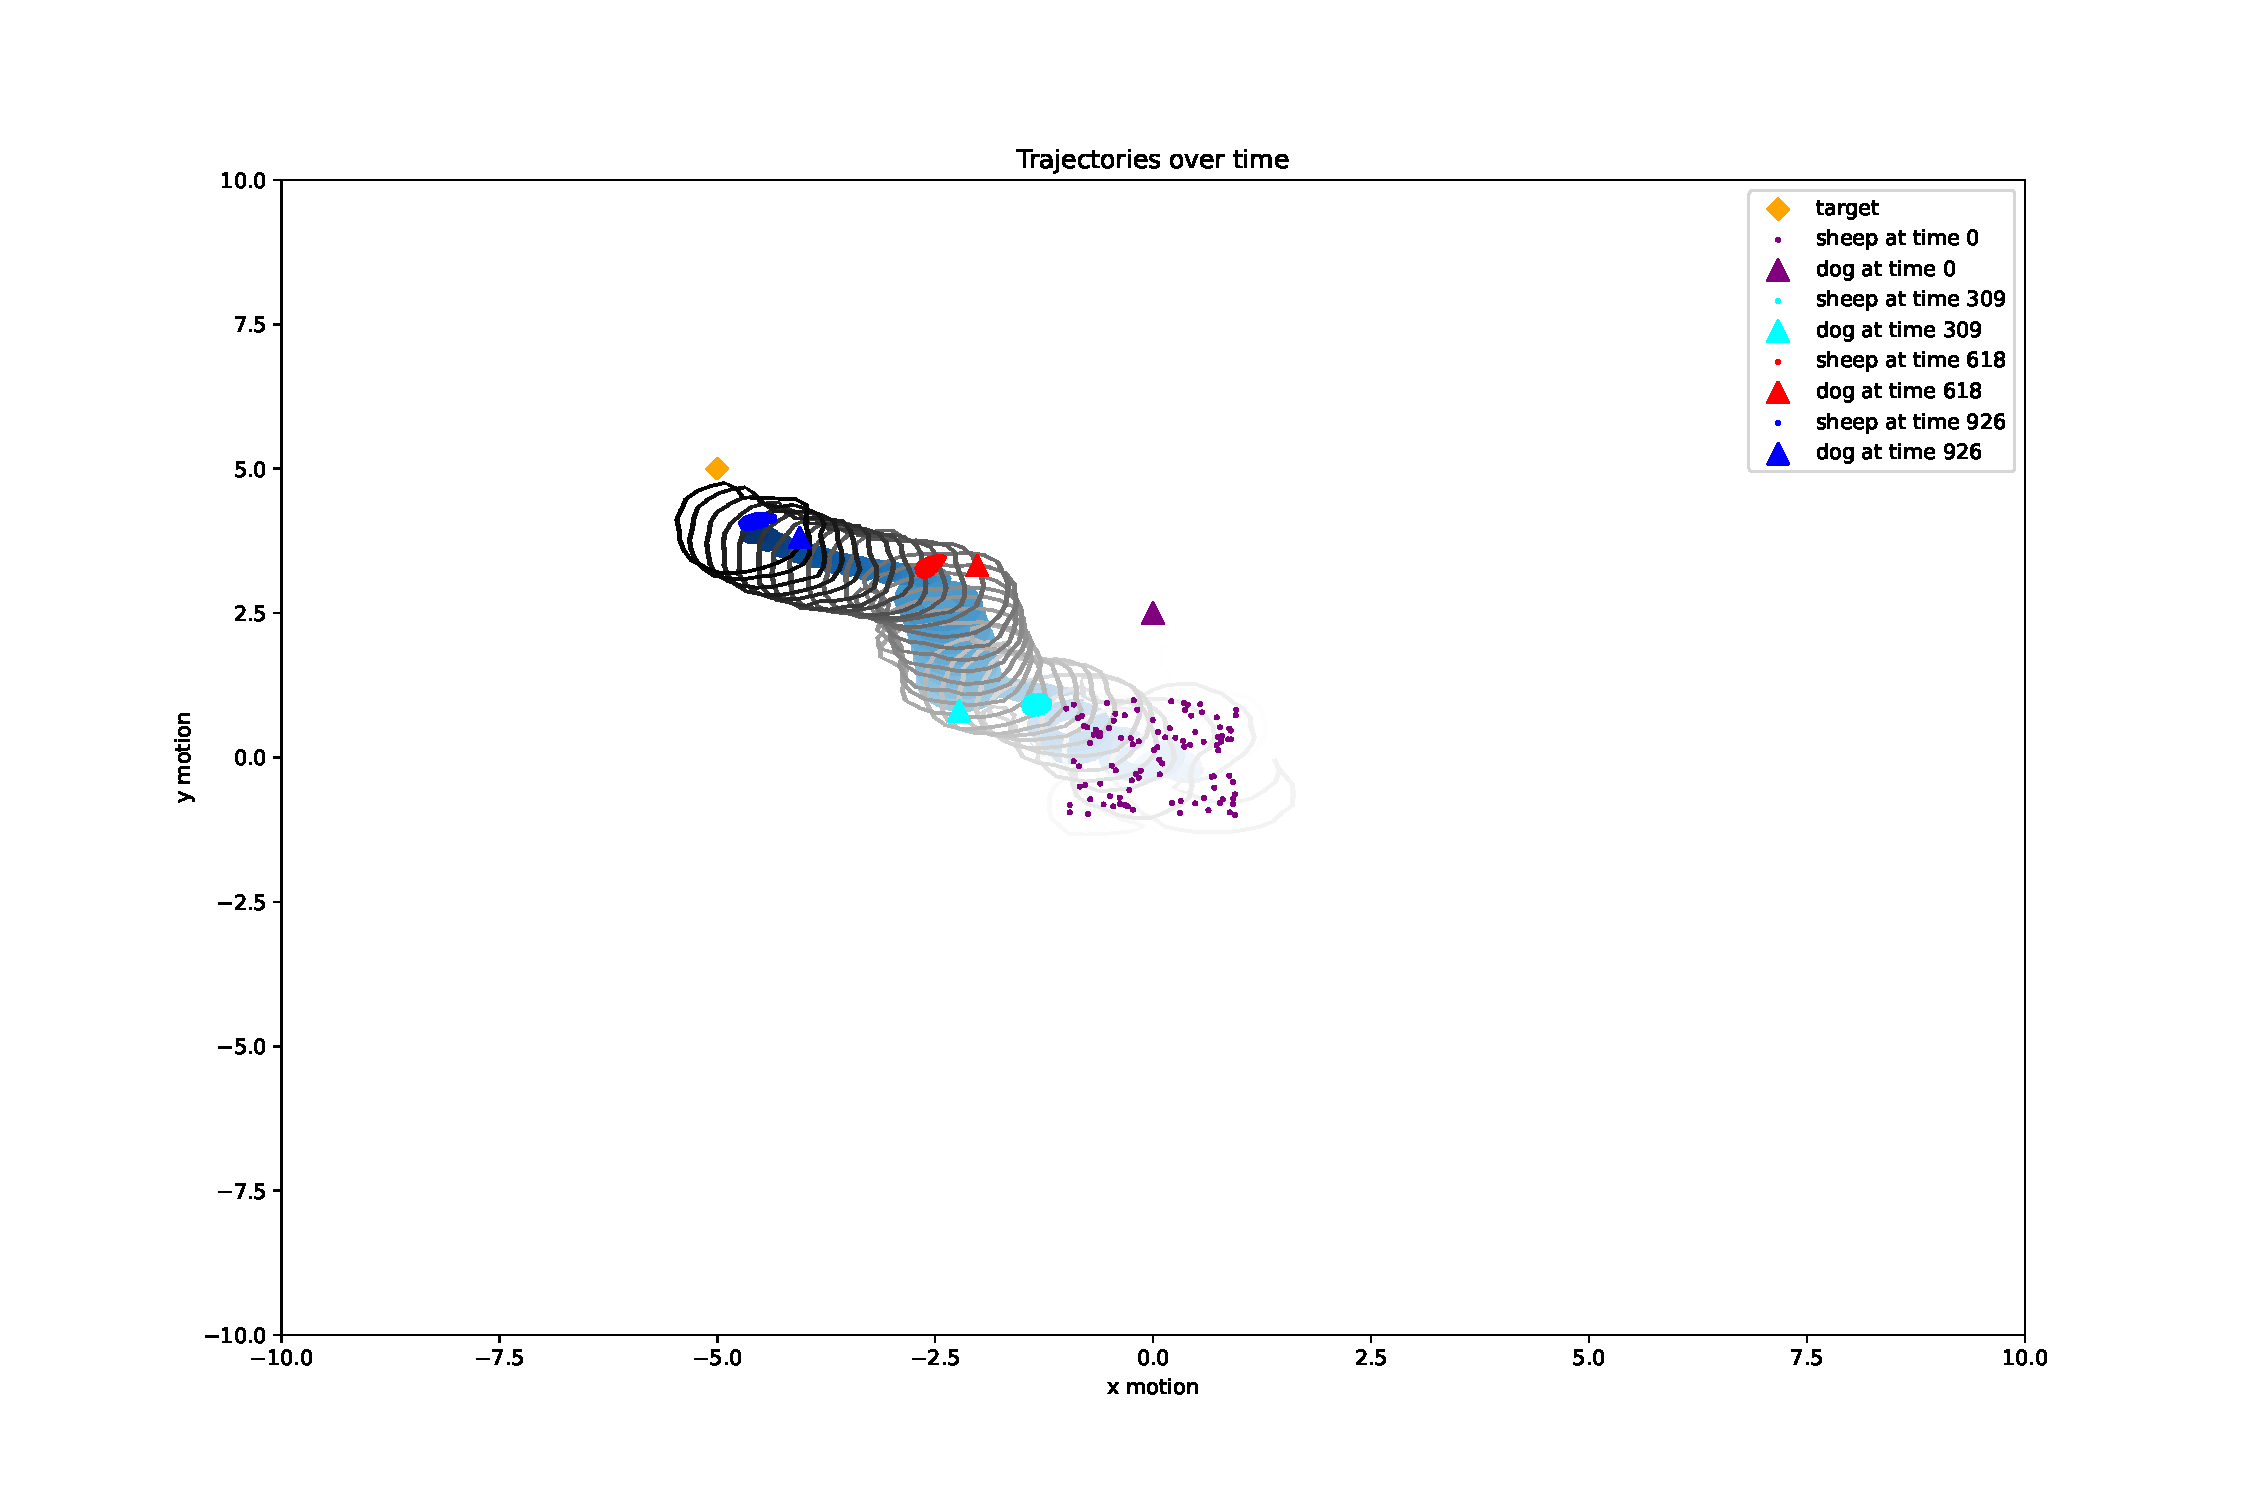
\includegraphics[width=\textwidth]{figures/mustering.pdf}
%     \caption{}
%   \end{minipage}
%   \hfill
%   \begin{minipage}[b]{0.49\textwidth}
%     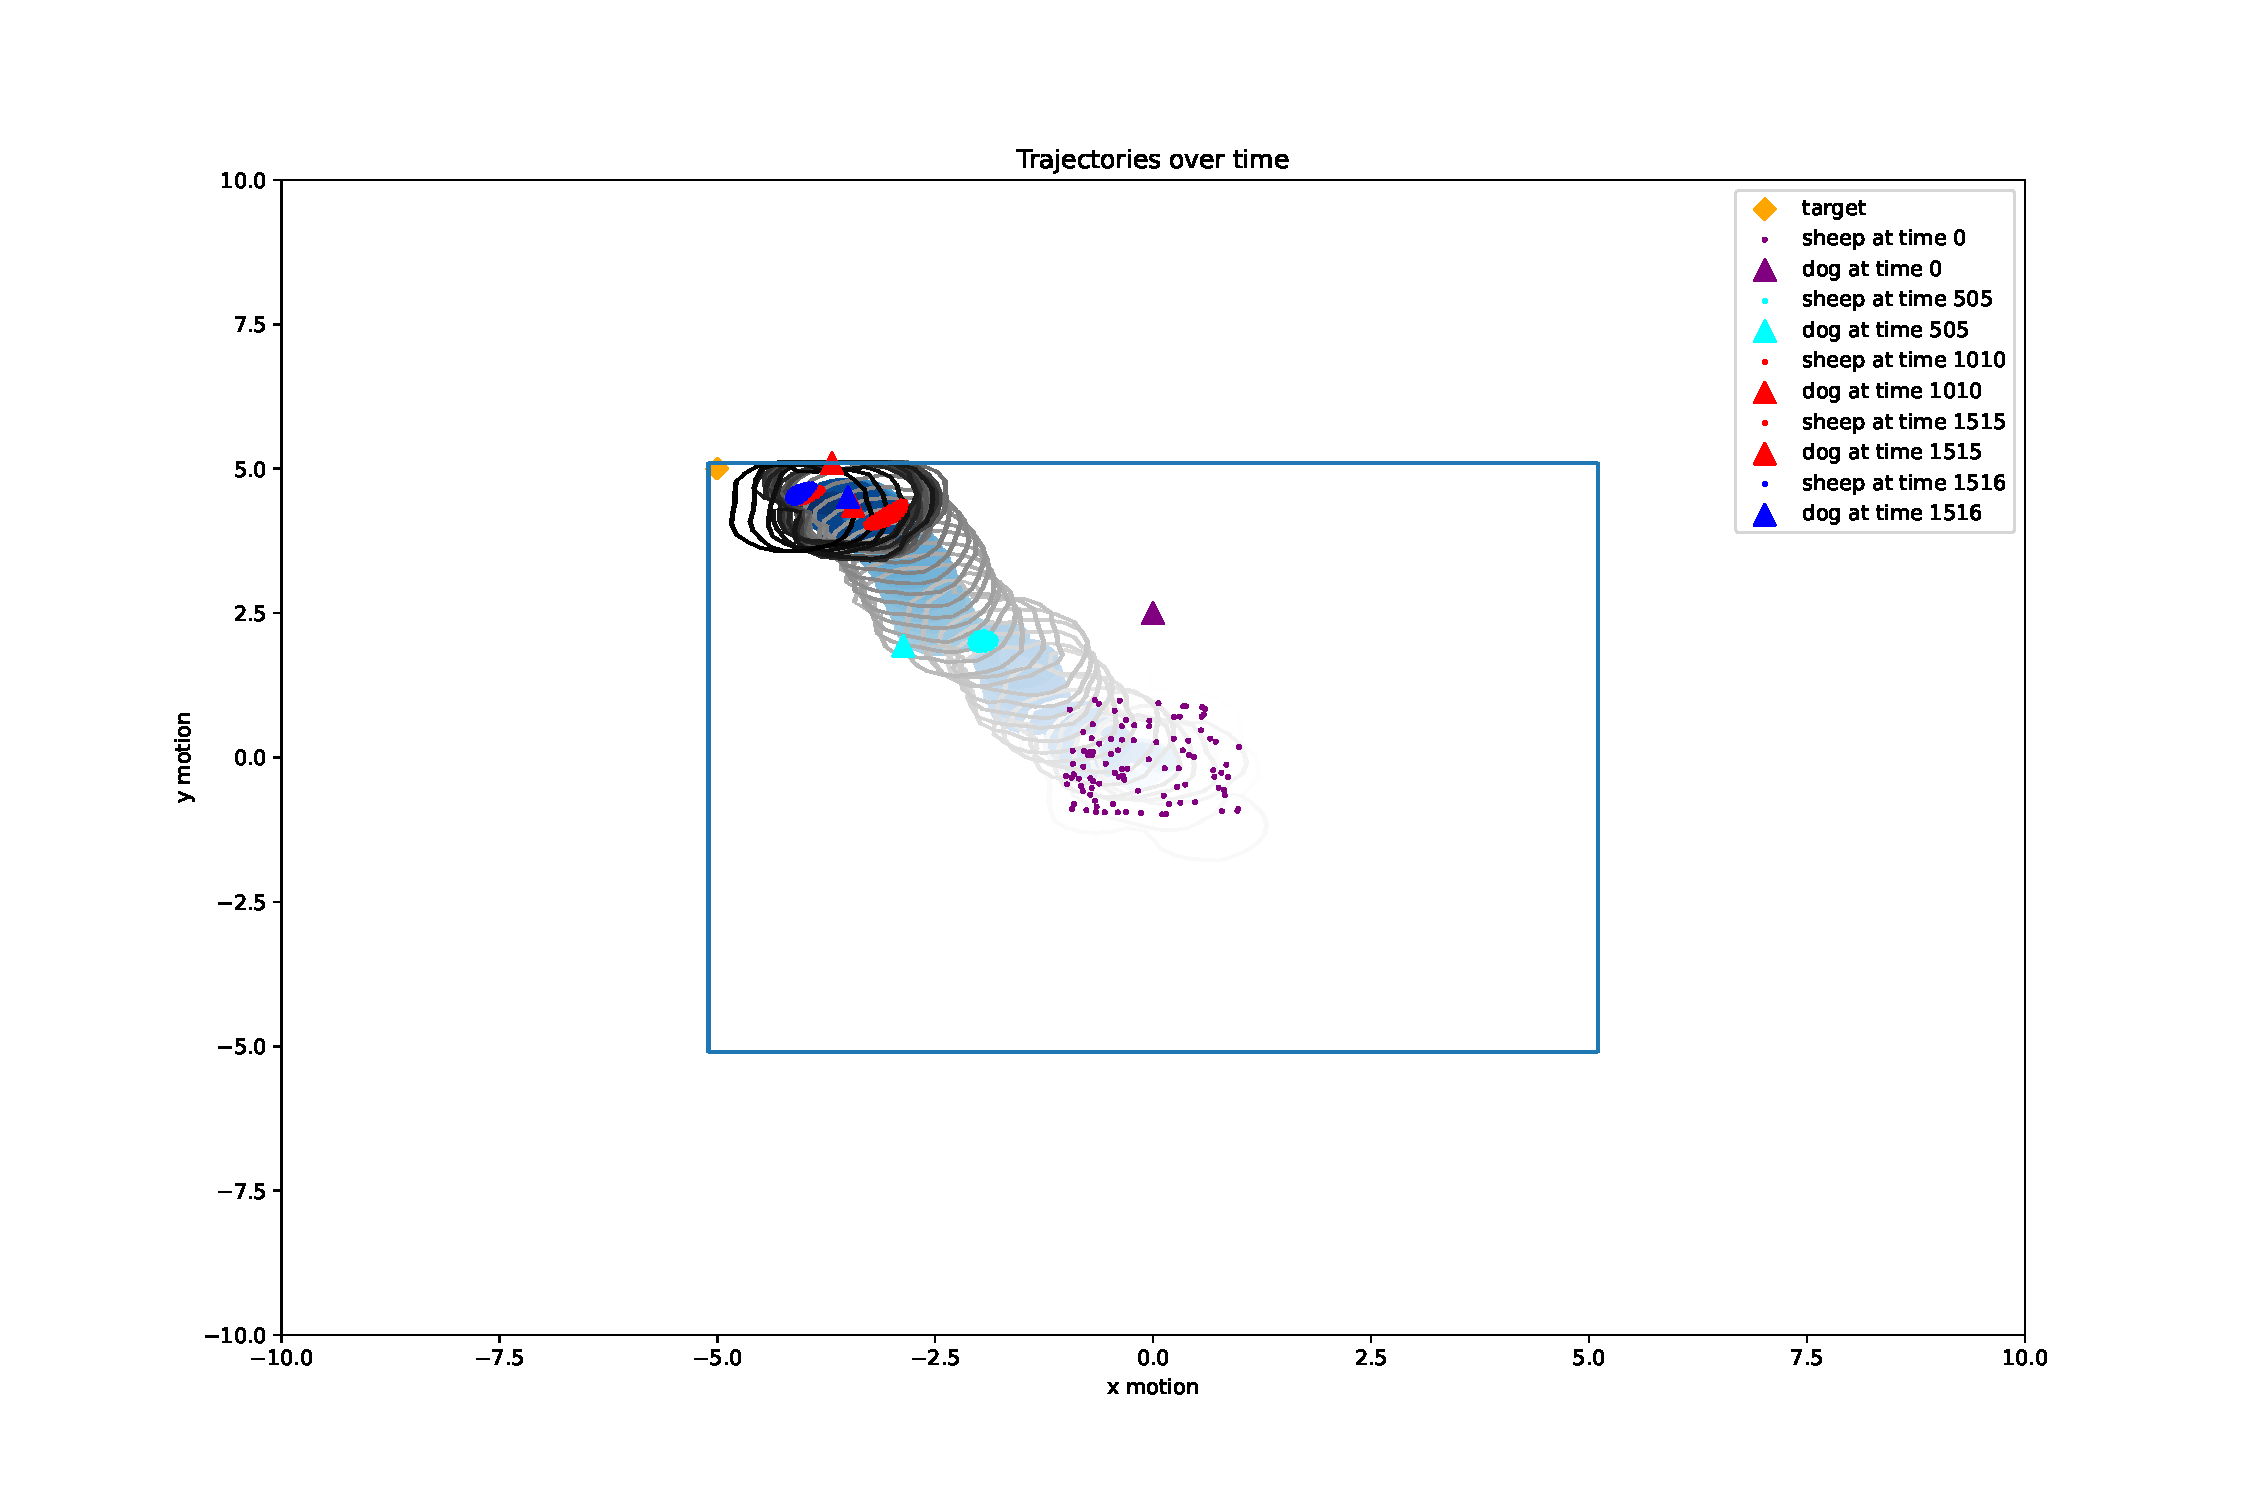
\includegraphics[width=\textwidth]{figures/mustering-fence.pdf}
%     \caption{}
%   \end{minipage}
% \end{figure}
